%%%%%%%%%%%%%%%%%%%%%%%%%%%%%%%%%%%%%%%%%%%%%%%%%%%%%%%%%%%%%%%%%%%%%%%%%%%%%%%%%%%%%%%%%%%%%%%%%%%
%
% Primordial Machine's Math Non Scalars Library
% Copyright (C) 2017-2019 Michael Heilmann
%
% This software is provided 'as-is', without any express or implied warranty.
% In no event will the authors be held liable for any damages arising from the
% use of this software.
%
% Permission is granted to anyone to use this software for any purpose,
% including commercial applications, and to alter it and redistribute it
% freely, subject to the following restrictions:
%
% 1. The origin of this software must not be misrepresented;
%    you must not claim that you wrote the original software.
%    If you use this software in a product, an acknowledgment
%    in the product documentation would be appreciated but is not required.
%
% 2. Altered source versions must be plainly marked as such,
%    and must not be misrepresented as being the original software.
%
% 3. This notice may not be removed or altered from any source distribution.
%
%%%%%%%%%%%%%%%%%%%%%%%%%%%%%%%%%%%%%%%%%%%%%%%%%%%%%%%%%%%%%%%%%%%%%%%%%%%%%%%%%%%%%%%%%%%%%%%%%%%

\documentclass[oneside]{book}

%%%%%%%%%%%%%%%%%%%%%%%%%%%%%%%%%%%%%%%%%%%%%%%%%%%%%%%%%%%%%%%%%%%%%%%%%%%%%%%%%%%%%%%%%%%%%%%%%%%
%
% Primordial Machine Math Non Scalars Library
% Copyright (c) 2017-2019 Michael Heilmann <michaelheilmann@primordialmachine.com>
%
% This software is provided 'as-is', without any express or implied warranty.
% In no event will the authors be held liable for any damages arising from the
% use of this software.
%
% Permission is granted to anyone to use this software for any purpose,
% including commercial applications, and to alter it and redistribute it
% freely, subject to the following restrictions:
%
% 1. The origin of this software must not be misrepresented;
%    you must not claim that you wrote the original software.
%    If you use this software in a product, an acknowledgment
%    in the product documentation would be appreciated but is not required.
%
% 2. Altered source versions must be plainly marked as such,
%    and must not be misrepresented as being the original software.
%
% 3. This notice may not be removed or altered from any source distribution.
%
%%%%%%%%%%%%%%%%%%%%%%%%%%%%%%%%%%%%%%%%%%%%%%%%%%%%%%%%%%%%%%%%%%%%%%%%%%%%%%%%%%%%%%%%%%%%%%%%%%%

\usepackage[utf8]{inputenc}
%
\usepackage{xparse}
\setcounter{tocdepth}{4} % Include subsubsections into ToC.
\setcounter{secnumdepth}{4} % Number subsubsection.
%
\usepackage{textcomp} % for \textlangle and \textrangle macros
\usepackage{xcolor}
%
\usepackage{xifthen}
%
\usepackage{datetime}
%
\usepackage{tabularx} % for tabularx environment
\usepackage{multirow}
%
\usepackage{lmodern}
\usepackage{microtype}
%
\usepackage{graphicx}
\usepackage[colorlinks]{hyperref}
\usepackage[margin=0.75in]{geometry}
\usepackage{amsmath,amssymb,amsfonts}

\setlength{\parindent}{0pt} % Disable paragraph indention.

\makeatletter

% "(Get|Set)Author".
% The name of the author.
\def\SetAuthor#1{\gdef\@author{#1}}
\def\@author{\@latex@warning@no@line{No author given}}
\def\GetAuthor{\@author}

% "(Get|Set)Email".
% The email (address) of the author.
\def\SetEmail#1{\gdef\@email{#1}}
\def\@email{\@latex@warning@no@line{No email given}}
\def\GetEmail{\@email}

% "(Get|Set)Organization".
% The organization the library is published by.
\def\SetOrganization#1{\gdef\@organization{#1}}
\def\@organization{\@latex@warning@no@line{No organization given}}
\def\GetOrganization{\@organization}

% "(Get|Set)LibraryName".
% The name of the library.
\def\SetLibraryName#1{\gdef\@libraryName{#1}}
\def\@libraryName{\@latex@warning@no@line{No library name given}}
\def\GetLibraryName{\@libraryName}

% "(Get|Set)LibraryIncludesPath".
% The includes directory path.
% Example: "primordialmachine/arithmetic-functors/$(PlatformTarget.toLower())/$(Configuration.toLower())/includes"
\def\SetLibraryIncludesDirectoryPath#1{\gdef\@libraryIncludesDirectoryPath{#1}}
\def\@libraryIncludesDirectoryPath{\@latex@warning@no@line{No library includes directory path given}}
\def\GetLibraryIncludesDirectoryPath{\@libraryIncludesDirectoryPath}

% "(Get|Set)LibraryIncludeFile".
% The include file name of the library.
% Example: "include.hpp".
\def\SetLibraryIncludeFileName#1{\gdef\@libraryIncludeFileName{#1}}
\def\@libraryIncludeFileName{\@latex@warning@no@line{No library include file name given}}
\def\GetLibraryIncludeFileName{\@libraryIncludeFileName}

% "(Get|Set)LibraryIncludeDirectiveFilePath".
% The library include directive file path.
% Example: "primordialmachine/arithmetic_functors/include.hpp".
\def\SetLibraryIncludeDirectiveFilePath#1{\gdef\@libraryIncludeDirectiveFilePath{#1}}
\def\@libraryIncludeDirectiveFilePath{\@latex@warning@no@line{No library include directive file path}}
\def\GetLibraryIncludeDirectiveFilePath{\@libraryIncludeDirectiveFilePath}

% "(Get|Set)LibraryStaticLibrariesDirectoryPath".
% The static libraries directory path.
% Example: "primordialmachine/arithmetic-functors/$(PlatformTarget.toLower())/$(Configuration.toLower())/libraries".
\def\SetLibraryStaticLibrariesDirectoryPath#1{\gdef\@libraryStaticLibrariesDirectoryPath{#1}}
\def\@libraryStaticLibrariesDirectoryPath{\@latex@warning@no@line{No library static libraries directory path given}}
\def\GetLibraryStaticLibrariesDirectoryPath{\@libraryStaticLibrariesDirectoryPath}

% "(Get|Set)LibraryStaticLibraryFileName.
% The static library file name of the library.
% Example: "arithmetic-functors.hpp".
\def\SetLibraryStaticLibraryFileName#1{\gdef\@libraryStaticLibraryFileName{#1}}
\def\@libraryStaticLibraryFileName{\@latex@warning@no@line{No library static library file name given}}
\def\GetLibraryStaticLibraryFileName{\@libraryStaticLibraryFileName}

% "(Get|Set)LibraryVersion".
% The version of the library.
\def\SetLibraryVersion#1{\gdef\@libraryVersion{#1}}
\def\@libraryVersion{\@latex@warning@no@line{No library version given}}
\def\GetLibraryVersion{\@libraryVersion}

% "(Get|Set)LibraryRepository".
% The repository (url) of the library.
\def\SetLibraryRepository#1{\gdef\@libraryRepository{#1}}
\def\@libraryRepository{\@latex@warning@no@line{No library repository given}}
\def\GetLibraryRepository{\@libraryRepository}

% "(Get|Set)DocumentType".
% The document type of this document.
\def\SetDocumentType#1{\gdef\@documentType{#1}}
\def\@documentType{\@latex@warning@no@line{No document type given}}
\def\GetDocumentType{\@documentType}

\let\tableofcontentsORIG\tableofcontents
\renewcommand\tableofcontents{\tableofcontentsORIG}

% Define "maketitle".
\def\maketitle{%
  \thispagestyle{empty}
  \begin{centering}

  \vspace*{6.0\baselineskip} % White space at the top of the page

  %%%%%%%%%%%%%%%%%%%%%%%%%%%%%%%%
  % TITLE
  %%%%%%%%%%%%%%%%%%%%%%%%%%%%%%%%

  \rule{\textwidth}{1.6pt}\vspace*{-\baselineskip}\vspace*{2pt} % Thick horizontal rule
  \rule{\textwidth}{0.4pt} % Thin horizontal rule

  \vspace{0.75\baselineskip} % Whitespace above the title

  {\normalsize\uppercase{\GetOrganization{}}'s}\\
  \vspace{1\baselineskip} % For some reason the lines are overlapping.
  {\LARGE\uppercase{\GetLibraryName} \uppercase{\GetLibraryVersion}}

  \vspace{0.75\baselineskip} % Whitespace below the title

  \rule{\textwidth}{0.4pt}\vspace*{-\baselineskip}\vspace{3.2pt} % Thin horizontal rule
  \rule{\textwidth}{1.6pt} % Thick horizontal rule

  \vspace{2\baselineskip} % Whitespace after the title block

  %%%%%%%%%%%%%%%%%%%%%%%%%%%%%%%%%
  % SUBTITLE
  %%%%%%%%%%%%%%%%%%%%%%%%%%%%%%%%%

  \vspace{2\baselineskip} % Whitespace after the title block

  \GetDocumentType % Subtitle or further description

  \vspace*{3\baselineskip} % Whitespace under the subtitle

  %%%%%%%%%%%%%%%%%%%%%%%%%%%%%%%%%
  % EDITORS
  %%%%%%%%%%%%%%%%%%%%%%%%%%%%%%%%%

  \vspace*{1\baselineskip} % Whitespace before editors

  Edited By

  \vspace{0.5\baselineskip} % Whitespace before the editors

  {\scshape\Large \GetAuthor \\
  {\normalsize(\href{mailto:\GetEmail}{\GetEmail})} \\} % Editor list

  \end{centering}

  %%%%%%%%%%%%%%%%%%%%%%%%%%%%%%%%%%
  % Footer
  %%%%%%%%%%%%%%%%%%%%%%%%%%%%%%%%%%
  \vspace*{\fill} % Whitespace before the editors
  \begin{tabularx}{\columnwidth}{m{0.75cm}m{4.75cm}X}
  \multirow{2}{=}{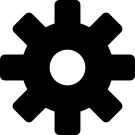
\includegraphics[scale=0.05]{primordialmachine-135x135.png}} & Primordial Machine                                                  & \hfill Created with \LaTeX\\
                                                                               & \href{https://primordialmachine.com}{https://primordialmachine.com} & \hfill Compiled on \today\ at \currenttime
  \end{tabularx}
}

\makeatother

\SetOrganization{Primordial Machine}
\SetLibraryName{Math Non Scalars}
\SetLibraryVersion{1.2}
\SetLibraryRepository{https://github.com/primordialmachine/math-non-scalars}
\SetAuthor{Michael Heilmann}
\SetEmail{michaelheilmann@primordialmachine.com}


\SetLibraryIncludeFileName{include.hpp}
\SetLibraryIncludesDirectoryPath{primordialmachine/math-non-scalars/\newline\$(PlatformTarget.toLower())/\$(Configuration.toLower())/includes}

\SetLibraryIncludeDirectiveFilePath{primordialmachine/math/non\_scalars/include.hpp}

\SetLibraryStaticLibrariesDirectoryPath{primordialmachine/math/non-scalars/\newline\$(PlatformTarget.toLower())/\$(Configuration.toLower())/libraries}
\SetLibraryStaticLibraryFileName{math-non-scalars.lib}

\SetDocumentType{User Manual}

\usepackage[listings,theorems]{tcolorbox}
\tcbset{before={\par\medskip\pagebreak[0]\noindent},after={\par\medskip}}%
\newcounter{example}[section]

\begin{document}

\frontmatter

\begin{titlepage}
\maketitle
\end{titlepage}

\tableofcontents
\addtocontents{toc}{\protect\thispagestyle{empty}}
\pagenumbering{gobble}

\mainmatter

\chapter{Synopsis}
C++ 17 library providing concepts and traits related to mathematical non-scalar types.
The library is made available publicly on
\href{\GetLibraryRepository}{Github}
under the
\href{\GetLibraryRepository/blob/master/LICENSE}{MIT License}.

\chapter{Limitations and Restrictions}
The library officially only supports Visual Studio 2017 and Windows 10.

\chapter{Introductory example}
\textit{\color{orange}This library does not provide any examples yet.}
%Examples are located in the \href{\GetLibraryRepository/blob/master/examples}{examples} directory.

%%%%%%%%%%%%%%%%%%%%%%%%%%%%%%%%%%%%%%%%%%%%%%%%%%%%%%%%%%%%%%%%%%%%%%%%%%%%%%%%%%%%%%%%%%%%%%%%%%%
%
% Primordial Machine's Math Indices Library
% Copyright (C) 2017-2019 Michael Heilmann
%
% This software is provided 'as-is', without any express or implied warranty.
% In no event will the authors be held liable for any damages arising from the
% use of this software.
%
% Permission is granted to anyone to use this software for any purpose,
% including commercial applications, and to alter it and redistribute it
% freely, subject to the following restrictions:
%
% 1. The origin of this software must not be misrepresented;
%    you must not claim that you wrote the original software.
%    If you use this software in a product, an acknowledgment
%    in the product documentation would be appreciated but is not required.
%
% 2. Altered source versions must be plainly marked as such,
%    and must not be misrepresented as being the original software.
%
% 3. This notice may not be removed or altered from any source distribution.
%
%%%%%%%%%%%%%%%%%%%%%%%%%%%%%%%%%%%%%%%%%%%%%%%%%%%%%%%%%%%%%%%%%%%%%%%%%%%%%%%%%%%%%%%%%%%%%%%%%%%

\chapter{Building under Visual Studio 2017}
\begin{enumerate}
\item Open the solution \texttt{solution.sln} in Microsoft Visual Studio 2017.
\item Batch build everything.
\item The folder \texttt{packages} contains the distribution of the library i.e. include files and the
      static libraries for
  \begin{enumerate}
    \item the platform targets \texttt{x86} and \texttt{x64} and
    \item configurations \texttt{Release} and \texttt{Debug}.
  \end{enumerate}
\item Copy the contents of the \verb+packages+ folder into a directory. Let
      \verb+[library home]+ be a placeholder denoting the path by which that folder
      can be referenced from your project.
\item Add
  \begin{enumerate}
    \item the include path
\texttt{[library home]/\GetLibraryIncludesDirectoryPath}
	and
    \item the library path
\texttt{[library home]/\GetLibraryStaticLibrariesDirectoryPath}
    to your project.
\end{enumerate}
\item Link your project with the library \texttt{\GetLibraryStaticLibraryFileName}.
\item Add the include directive \texttt{\#include "{}\GetLibraryIncludeDirectiveFilePath"{}} where appropriate.
\item You can now use the functionality provided by the library.
\end{enumerate}


\chapter{Library Interface Documentation}

\section{\texttt{namespace primordialmachine}}
The namespace this library is adding its declarations/definitions to.
The added namespace elements are documented below.

\section{\textit{Math.NonScalar} (type concept)}
A \textit{Math.NonScalar} type is a fixed size container for   \textit{Math.Scalar}
type elements which can be accessed for reading an writing using different indexing
schemes. Matrices, points, and vectors are examples of      \textit{Math.NonScalar}
types. 

\subsection{Element type}
The \textit{Math.Scalar} type $E$ of the elements of a \textit{Math.NonScalar} type
$T$ can be obtained by the member type definition\newline
\texttt{element\_type\textlangle $T$\textrangle::type}\newline
or the type definition\newline
\texttt{element\_type\_t\textlangle$T$\textrangle}\newline

\subsection{Number of elements}
The number of elements of a \textit{Math.NonScalar} type $T$ can be obtained by
the constant expression \textit{size\_t} member constant\newline
\texttt{number\_of\_elements\textlangle $T$\textrangle::value}\newline
or by the constant expression \textit{size\_t} constant\newline
\texttt{number\_of\_elements\_v\textlangle $T$\textrangle}\newline

\subsection{Degenerate and non-degenerate}
A \textit{Math.NonScalar} type $T$ called \textit{degenerate} if and only if it has zero elements.
Otherwise it is called \textit{non-degenerate}.

If a \textit{Math.NonScalar} type $T$ is degenerate can be obtained by
the constant expression \textit{bool} member constant\newline
\texttt{is\_degenerate\textlangle $T$\textrangle::value}\newline
or by the constant expression \textit{bool} constant\newline
\texttt{is\_degenerate\_v\textlangle $T$\textrangle}\newline

If a \textit{Math.NonScalar} type $T$ is non-degenerate can be obtained by
the constant expression \textit{bool} member constant\newline
\texttt{is\_non\_degenerate\textlangle $T$\textrangle::value}\newline
or by the constant expression \textit{bool} constant\newline
\texttt{is\_non\_degenerate\_v\textlangle $T$\textrangle}\newline

\subsection{Dimensionality $=0$}
A \textit{Math.NonScalar} of dimensionality $=0$ is a type $T$
which provides support for the following   operations:\newline

%BEGIN OPERATIONS%
\texttt{$T$(const $T$\& other)}\textit{(copy constructor)}\newline
\texttt{$T$\& operator=(const $T$\& other)}\textit{(copy assignment operator)}\newline
%END OPERATIONS%

\subsection{Dimensionality $=1$}
A \textit{Math.NonScalar} of dimensionality $=1$ provides the     same
operations as a \textit{Math.NonScalar} type of   dimensionality $=0$.
In addition, it provides support for the following operations:\newline

%BEGIN OPERATIONS%
\texttt{const element\_type\& operator()(size\_t i) const}\textit{(constant unary indexing operator})\newline
\texttt{element\_type\& operator()(size\_t i)} \textit{(unary indexing operator)}\newline
%END OPERATIONS%

\subsection{Dimensionality $>1$}
A \textit{Math.NonScalar} of dimensionality $>1$ provides the     same
operations as a \textit{Math.NonScalar} type of   dimensionality $=1$.
In addition, it provides support for the following operations:\newline

%BEGIN OPERATIONS%
\texttt{const element\_type\& operator()(\textit{IndexList}) const} \textit{(constant $n > 1$-ary indexing operator)}\newline
\texttt{element\_type\& operator()(\textit{IndexList})} \textit{($n > 1$-ary indexing operator)}\newline
%END OPERATIONS%

where \texttt{\textit{IndexList}} are $n$ \texttt{size\_t} values
denoting indices and where $n$ is the dimensionality of      $T$.\newline

Every \textit{Math.NonScalar} of dimensionality $n > 1$     must define a
bijection between the indices $i$ passed to the unary \texttt{operator()}
and the indices $i_0,\ldots,i_{n-1}$ passed to the            $n > 1$-ary
\texttt{operator()}.\newline

\begin{tcolorbox}[title=Example]
Row-major $N \times M$ matrices where $N$ is the   number of
rows and $M$ is the number of columns can fulfil         the
\textit{Math.NonScalar} type concept of  dimensionality $2$:
First, provide th $2$ index operators such that the first
index denotes the row index and the second index      the
column index.
Second, provide the $1$ index   operators and define the
bijection between an index $i$ passed to the $1$   index
operator and the first index $j$   and the second index:
A possible bijection can be defined in terms of a    row
major mapping as $k$ as $i / N + i\mod M= j \cdot M +k$.
\end{tcolorbox}

\subsection{Number of elements}
\textcolor{orange}{To be done.}

%%%%%%%%%%%%%%%%%%%%%%%%%%%%%%%%%%%%%%%%%%%%%%%%%%%%%%%%%%%%%%%%%%%%%%%%%%%%%%%%%%%%%%%%%%%%%%%%%%%
\section{\texttt{index\_1} (struct)}
A \texttt{struct} representing a one dimensional index.

\subsection{Constructors}
\subsubsection{\texttt{index\_1(size\_t i)}}
\texttt{constexpr index\_1(size\_t i)}\newline
Contruct this \texttt{index\_1} object with the specified index.

\subsection{Methods}
\subsubsection{\texttt{i()}}
\texttt{constexpr const size\_t\& i() const}\newline
\texttt{constexpr size\_t\& i()}\newline
Method returning the index \texttt{i}.

%%%%%%%%%%%%%%%%%%%%%%%%%%%%%%%%%%%%%%%%%%%%%%%%%%%%%%%%%%%%%%%%%%%%%%%%%%%%%%%%%%%%%%%%%%%%%%%%%%%
\section{\texttt{index\_2} (struct)}
A \texttt{struct} representing a two dimensional index.

\subsection{Constructors}
\subsubsection{\texttt{index\_2(size\_t i, size\_t j)}}
\texttt{index\_1(size\_t i, size\_t j)}\newline
Contruct this \texttt{index\_2} object with the specified indices.

\subsection{Methods}
\subsubsection{\texttt{i()}}
\texttt{constexpr const size\_t\& i() const}\newline
\texttt{constexpr size\_t\& i()}\newline
Method returning the index \texttt{i}.

\subsubsection{\texttt{j()}}
\texttt{constexpr const size\_t\& j() const}\newline
\texttt{constexpr size\_t\& j()}\newline
Method returning the index \texttt{i}.

\end{document}
